
% Functionality
HBase is a distributed key-value store that is part of the Hadoop open source  technology suite. 
It is implemented in Java. Similarly to other modern KV-stores, HBase follows the design of 
Google's Bigtable~\cite{Chang2008}. We sketch out their common design principles 
and terminology. 

\paragraph{Data model}
KV-stores hold data items referred to as \emph{rows} identified by unique 
row keys. Each row can consist of multiple \emph{columns} (sometimes called fields) identified by unique 
column keys. Co-accessed columns (typically used by the same application) can be 
aggregated into  \emph{column families} to optimize access. The data is multi-versioned, 
i.e., multiple versions of the same row key can exist, each identified by a unique {\em timestamp}. 
The smallest unit of data, named {\em cell}, is defined by a combination of a row key, a
column key, and a timestamp.

The basic KV-store API includes \emph{put} (point update of one or more cells, by row key), 
\emph{get} (point query of one or more columns, by row key, and possibly column keys), 
and \emph{scan} (range query of one or more columns, of all keys between 
an ordered pair of begin and end row keys). 

\begin{figure}[tb]
\center
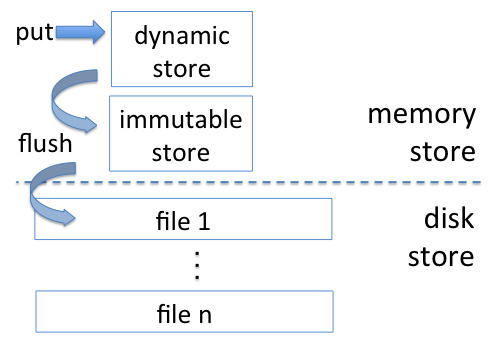
\includegraphics[width=0.9\columnwidth]{LSM} 
\caption{A log-structured merge (LSM) tree consists of a small memory store ({\em MemStore} in HBase) 
and a large disk store (collection of {\em HFiles}). Put operations update the MemStore. The latter is 
double-buffered: a flush creates an immutable \emph{snapshot} of the active buffer and  a new active 
buffer. The snapshot is then written to disk in the background.}
\label{fig:LSM}
\end{figure}

\paragraph{Data management}
KV-stores achieve scalability by sharding tables into range partitions by row key. 
A shard is called {\em region\/} in HBase (\emph{tablet} in Bigtable). 
A region is a collection of \emph{stores}, each associated with a column family. 
Each store is backed by a collection of files sorted by row key, called \emph{HFiles} in HBase 
(\emph{sst files} in Bigtable). 

In production, HBase is typically layered on top of Hadoop Distributed Filesystem (HDFS), 
which provides a reliable file storage abstraction. HDFS and HBase normally share the same hardware. 
Both scale horizontally to thousands of nodes. HDFS replicates data for availability (3-way by default). 
It is optimized for very large files (the default block size is $64$MB).

Data access in HBase is provided through {\em region servers} (analogous to {\em tablet servers}
in Bigtable). Each region server controls multiple stores (tens to hundreds in production settings). 
For locality of access, the HBase management plane (\emph{master server}) tries to lay out the 
HFiles in HDFS so that their primary replicas are collocated with the region servers that control them. 

\paragraph{LSM trees}
Each store is organized as an LSM tree, which collects writes in a memory store --
\emph{MemStore} in HBase -- and periodically flushes the memory into a disk store, as illustrated in 
Figure~\ref{fig:LSM}. Each flush creates a new immutable HFile, ordered by row key for query efficiency. 
HFiles are created big, hence flushes are relatively infrequent. 

To allow puts to proceed in parallel with I/O, MemStore employs double buffering:
it maintains a dynamic \emph{active} buffer absorbing puts, and a static \emph{snapshot}
that holds the previous version of the active buffer. The latter is written to the 
filesystem in the background. Both buffers are ordered by key, as are the HFiles.  

% LSM puts and flushes
A flush occurs  when either the active buffer 
exceeds the region size limit ($128$MB by default) or  the overall footprint of all MemStores
in the region server exceeds the global size limit ($40\%$ of the heap by default). 
Flush first shifts the current active buffer to be the snapshot (making it immutable) and creates a new empty active buffer.
It then replaces the reference to the active buffer, and proceeds to write the snapshot as a new HFile. 

% WAL
In order to guarantee durability of writes between flushes, updates are first written to 
a \emph{write-ahead log} (WAL). HBase implements the logical WAL as collection of one or more physical 
logs per region server, called \emph{HLogs}, each consisting of multiple log files on HDFS. 
As new data gets flushed to HFiles, the old log files become redundant, and the system collects 
them in the background. 
%On the other hand, 
If some HLog grows too big, the system may forcefully
flush the MemStore before the memory bound is reached, in order to enable the log's truncation. 
Since logged data is only required at recovery time and is only scanned sequentially, HLogs
may be stored on slower devices than HFiles in production (e.g., HDDs vs SSDs). 
Real-time applications often trade durability for speed by aggregating multiple log records 
in memory prior to asynchronously writing them to WAL in a bulk. 

To keep the number of HFiles per store bounded, \emph{compactions} merge multiple files 
into one, while eliminating redundant (overwritten) versions. If compactions cannot keep up
with the flush rate, HBase may either throttle or totally block  puts until  compactions 
successfully reduce the number of files. 

Most compactions are \emph{minor}, 
in the sense that they merge a subset of the HFiles. \emph{Major} compactions merge all the region's 
HFiles. Because they have a global view of the data, major compactions also eliminate 
{\em tombstone} versions that indicate row deletions. Typically, major compactions incur huge 
performance impact on concurrent operations. In production, they are either carefully scheduled 
or performed manually~\cite{hbasetuning}.

% LSM gets
The get operation searches for the key in parallel in the MemStore (both the active and the 
snapshot buffers) and in the HFiles. The HFile search  is expedited through Bloom 
filters~\cite{Chang2008}, which eliminate most redundant disk reads. The system 
uses a large RAM cache for popular HFile blocks (by default $40\%$ of the heap).

\paragraph{Memory organization}
The MemStore's active buffer is traditionally implemented as a dynamic index over a collection of cells.  
The HBase implementation uses the standard Java concurrent skiplist map~\cite{javaskiplist}.
Data is multi-versioned -- every put creates a new immutable version of the row it is applied to, 
consisting of one or more cells. 

This implementation suffers from two drawbacks. First, the use of a big dynamic data structure entails 
the abundance of auxiliary small objects and references, which inflate the in-memory index and induce 
a high GC cost. The overhead is most significant when the managed objects are small, i.e., 
the metadata-to-data ratio is big~\cite{Wu2015}. Second, the versioning mechanism 
makes no attempt to eliminate redundancies prior to flush, i.e., the MemStore size  steadily grows, 
independently of the workload. This is especially wasteful for heavy-tailed (e.g., power law) key access distributions, 
which are prevalent in production workloads~\cite{Devineni:2015}. 

The \sys\/ algorithm takes care of precisely these problems, to boost  
LSM tree performance and reduce  storage wear-out. Section~\ref{sec:accordion} 
presents it in detail. 







